\documentclass[main.tex]{subfiles}
% \nomenclature[A]{GPR}{Ground Penetrating Radar}%

\begin{document}
\chapter{Feasibility Study}
\chaplabel{literatureReview}
This chapter provides a summary of the benchmarking process, as detailed in \Chapref{benchmarking}, and then presents the literature review, which covers the areas of signal processing and sensor fusion, as well as navigation. \todo[inline]{\textbf{General comments for lit review: Very shallow, needs many more references, need to explain ``state of the art'', explain current level of understanding in this field }}

\section{Benchmarking}
Metal detectors are the most widely used sensor for manual landmine detection. While they are simple to operate, they are limited by the variety of landmine types they can detect. They also produce a large number of false positives, leading to demining operations being inefficient \parencite{minelabF3}. Another type of sensor that is increasingly used for manual landmine detection applications is the ground penetrating radar or GPR. These sensors allow small variations in density beneath the soil surface to be detected, meaning GPRs can be used to find metallic and non-metallic targets \parencite{sakaguchi2014}. However, this sensitivity makes it difficult to identify detected objects, especially in certain soil types. Multisensor systems, which for instance combine a metal detector and a GPR, allow the limitations of the individual systems to be addressed, leading to improved landmine detection performance \parencite{Takahashi10}. Whatever the sensor used, signal processing is an important requirement, particularly for the GPR. In the case of a multisensor system, sensor fusion must also be employed to consolidate the data from the individual sensors to provide meaningful output.  

An alternative to manual landmine detection methods is vehicle or platform based landmine detection. There are a wide variety of platform types used, a growing number of which have remote control or autonomous operation capabilities \parencite{portugal2014}. The selection of platform type largely depends on the sensor payload and scenario of operation. Key challenges regardless of the platform used include automation of the system, encompassing hardware and the control system, and navigation, which could have varying levels of complexity depending on the features to be implemented. 

\textcolor{red}{Need to add some references to the above paragraphs, grab them from the benchmarking appendix - RK}

\section{Signal processing}
As identified through benchmarking, signal processing is a major challenge associated with landmine detection. As part of the project, the outputs from both a metal detector and a GPR must processed. \textcolor{red}{Need to talk about challenges and relate to mission profile}
\seclabel{splitreview}

\subsection{Metal detector signal processing}
A metal detector utilises a transmitting source and a receiving device to detect subsurface objects. Metal detectors that operate on the eddy current principle generate magnetic fields which penetrate the soil, inducing eddy currents in underground metallic objects. These eddy currents in turn generate a secondary magnetic field, at a greatly reduced amplitude, which can then be detected by the receiving coil of the metal detector \parencite{Candy2008}. The signal to noise ratio obtained is often low, especially in heavily mineralised soils, and all signals are heavily attenuated with depth \parencite{Candy2008}.

Commercially available metal detectors convert the received signals directly to an audio signal, allowing an operator to distinguish different metal objects from the amplitude and tone of the received signal. Using this method, qualified demining personnel can readily locate the position of a subsurface object, however full classification of the object or determination of its characteristics, such as size, shape and material, are practically impossible \parencite{Kruger2006}. Some degree of basic automatic classification is common on devices marketed for treasure hunting, where it is used to distinguish valuable metallic objects from common metals. This classification is known as a discriminated signal, and is possible due to the variation in eddy currents induced by different metals - most particularly between ferrous and non-ferrous metals. 

% The signal response that allows the creation of the discriminated signal is the time constant of the received audio sample. The time constant is a function of the metallic material being detected, based largely on the target inductance and conductivity \parencite{Candy2008}. Selectively discriminating times when the signal's time constant meets a certain criteria allows for the detection of different metal types, with most ferrous targets having very long time constants, and targets composed of other metals being able to be discriminated based on expected time constant range \parencite{Candy2008}. This method however is not generally applicable to the purposes of landmine detection as the size and shape of a material can influence the time constant, and as such the method is not reliable for typical landmines, which consist of small parts of different materials and complex shapes \parencite{Kruger2006}. The influence of mineralised soil is also not compensated for by the discriminator which would also affect the determination of metal type \parencite{Kruger2006}.

A more appropriate method for landmine detection, and particularly automatic landmine detection, is to compare the phase plot signatures of landmines objects with a database of sample signatures. The phase plot signature of an object can be generated by representing the sample signal in the complex plane, an advantageous strategy as the required signal to noise ratio for a high quality signature is low \parencite{Kruger2006}. The phase plot signatures for several example objects are shown in \Figref{signature}, demonstrating the variance in signature between objects.
\begin{figure}[ht]
\centerline{
\begin{tabular}{cccc}
\subfloat[Landmine]{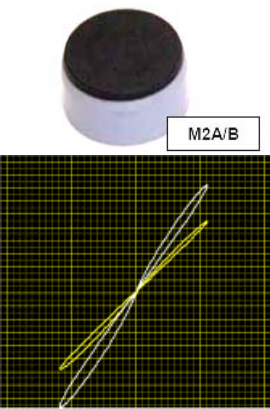
\includegraphics[width=0.21\textwidth]{2-LiteratureReview/S1.PNG}}
& \subfloat[Bullet casing]{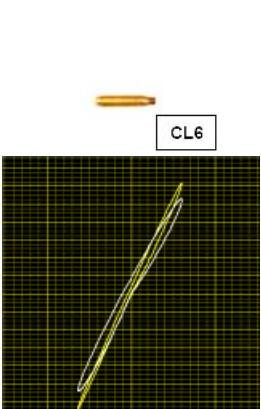
\includegraphics[width=0.21\textwidth]{2-LiteratureReview/S2.PNG}}
& \subfloat[Soft drink can]{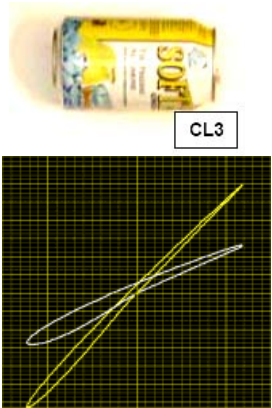
\includegraphics[width=0.21\textwidth]{2-LiteratureReview/S3.PNG}}
& \subfloat[Steel ball]{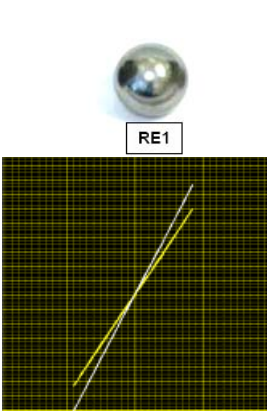
\includegraphics[width=0.21\textwidth]{2-LiteratureReview/S4.PNG}}\\
\end{tabular}}
\caption[Phase plot signatures of various subsurface objects]{Phase plot signatures of various subsurface objects in the complex plane, with the  \parencite{Kruger2006}}
\figlabel{signature}
\end{figure}

This signature is capable of uniquely identifying an object type to a certain degree, which allows for objects to be easily classified and hence identified. The low signal to noise ratio requirement also means that the strategy is reasonably robust against depth based attenuation, allowing the classification of objects irrespective of depth. This result is shown in \Figref{comp-signature}. \Figref{comp-signature} also highlights the requirement for ground signal compensation to allow for correct matching of signatures. It is important to note that the ground compensation algorithm used on the samples must be identical to the ground compensation algorithm used to generate the signatures from the training set to guarantee comparability \parencite{Kruger2006}.
\begin{figure}[ht]
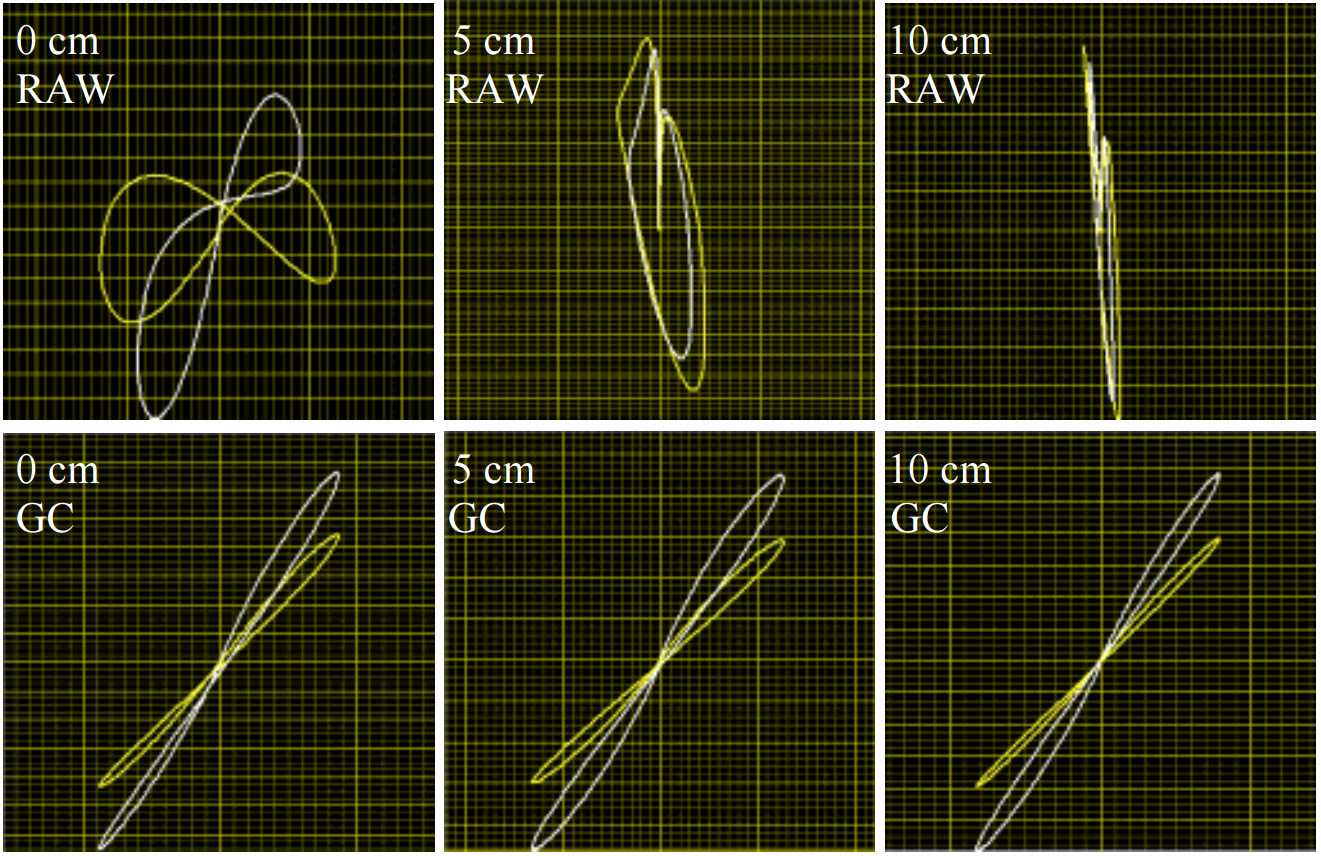
\includegraphics[width=0.8\textwidth]{2-LiteratureReview/compensated-signature.png}
\centering
\caption[Phase plot signatures of a landmine at varying depths]{Phase plot signatures of a landmine at varying depths. The top row shows the raw phase plots and the bottom row shows the phase plots after ground compensation, and the two loops in each image correspond to different frequencies \parencite{Kruger2006}} \figlabel{comp-signature}
\end{figure}

A notable failure of the phase plot signature method is the effect of nearby metallic objects. A metallic non-landmine object situated immediately next to a landmine can interfere with the signature of the received sample, reducing the likelihood that a correct identification will be made. This is particularly problematic for large metallic objects, which can completely obscure the signature of smaller objects. As a result, this technique is limited to situations in which metallic contamination is sparse, or metallic objects are typically an order of magnitude smaller than the objects of interest \parencite{Kruger2006}.

\textcolor{red}{If time permits and there are enough words left, go back and add more details about MD signal processing from Bruschini, since only two references are used here atm - RK}

\subsection{GPR signal processing}
\seclabel{gpr}
\subsubsection{Hardware configuration influence on detection capability}
\textcolor{red}{Maziar underlined this heading, not sure why... But this subsection isn't really about signal processing, can get rid of it or summarise it a lot.}

Ground penetrating radars operate by transmitting radio signals, and measuring the strength of reflected signals, caused by changes in density at the interface between objects and the soil \parencite{sakaguchi2014}. Achieving a high signal to noise ratio is a challenge with a GPR, as signal noise is introduced at all locations where even a small change in density occurs \parencite{shresta2003}. Thus, the primary challenge when searching for objects using GPR technology is being capable of distinguishing important objects from a noisy signal response \parencite{sakaguchi2014}.

Radar frequencies are attenuated by underground objects, as they absorb the energy in the transmitting signal, dampening the possible response to the receiving antenna. This is particularly apparent in certain soil types, notably wet soils and clays, which have a significant damping effect on the radar pulses \parencite{sakaguchi2014}.By increasing the power of the transmitted signal or increasing the gain on the receiving signal, the effects of ground attenuation can be reduced, allowing for greater scanning depth with a GPR \parencite{Ho2008}. Increasing the receiver gain also has the effect of amplifying any noise generated through the system, making the detection of subsurface objects heavily constrained by the ability to differentiate objects of interest from non-significant features \parencite{shresta2003}. 

Due to the attenuation of the radar signal through the soil, and the limits on the receiving signal gain, a trade-off exists between the maximum sensing depth and the detection resolution \parencite{Ho2008}. A solution to this is wideband frequency coverage, which makes use of the fact that different frequencies experience different levels of attenuation. A lower frequency transmitter and receiver, $\sim$200 MHz, will be capable of detecting at greater depths than a high frequency, at the sacrifice of detection resolution. Conversely high frequency systems, $\sim$3 GHz, will achieve greater resolution at the cost of severe attenuation with increased depth \parencite{shresta2003}. Wideband frequency coverage is the application of antennas which are capable of varying their frequency to allow a single device to scan over a wide frequency band. By collating detection results from multiple frequencies, a combined response can be created, which has signal responses from large, deep objects while retaining the ability to distinguish small objects at shallow depths \parencite{3dradarDXG}.

The detection of subsurface objects is effectively limited to objects situated between the transmitting and receiving antennas, which in practice must be only a small distance apart due to signal attenuation. This prevents the scanning of wide fields by placing the antennas a wide distance apart. Iterative scanning must be employed to cover a zone, and with a small scan width this requires a great number of scans. The limitation of a single radar scanline can be overcome with the use of an array of transmitting and receiving antennas combined into a single scanning device. Under this arrangement, the series of transmitting and receiving antennas are displaced laterally from each other along the length of the device, as represented by arrows in \Figref{arraylayout}. The effective sensing locations by pairing each receive antenna to two transmitting antennas are shown as dots in \Figref{arraylayout}. The application of multiple transmitting and receiving pairs allows for a single pass to scan a significant width, limited only by the number of transmitting and receiving pairs \parencite{3dradarDX}. 
\begin{figure}[ht]
\centering
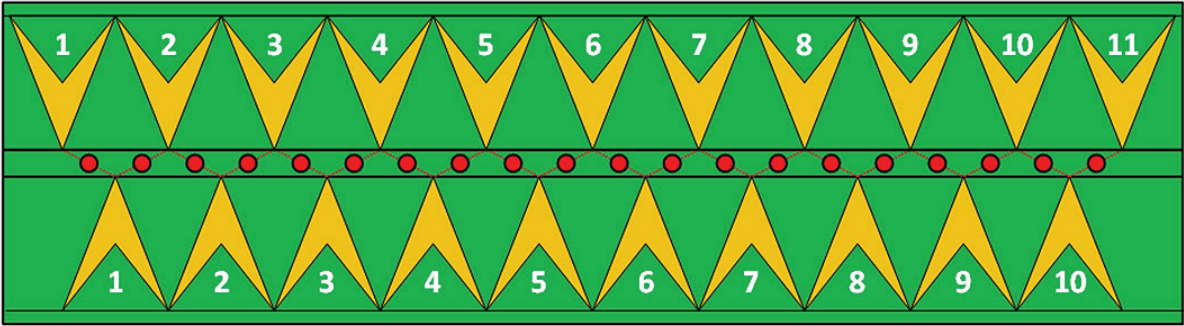
\includegraphics[width=0.8\textwidth]{2-LiteratureReview/3d-radar.png}
\caption[Layout of transmitting and receiving antennas of a GPR array]{Layout of transmitting (bottom row) and receiving antennas (top row) of a GPR array, with effective sensing locations shown as dots \parencite{3dradarDXG}}
\figlabel{arraylayout}
\end{figure}

\subsubsection{Signal processing and determination of objects of interest}
Typically there are three steps required to process GPR signals for landmine detection, \parencite{Ho.etal2004}:
\begin{itemize}
\item \textbf{Preprocessing}: Background signal removal and clutter suppression.
\item \textbf{Initial detection}: Selection of all suspicious anomalies present in the scan.
\item \textbf{Classification}: Analysing the data and determining which of the suspicious anomalies have a high likelihood of being a landmine.
\end{itemize}
The classification step requires determining a set of characteristics or metrics which suitably and uniquely identify the feature of an object of interest. These metrics are limited to those which can be accurately measured by the GPR device, and are commonly the size, shape and other physical aspects of the object \parencite{Ho2008}. However, objects can also be identified from the raw signal without the need to link parameters to real-world object characteristics, by identifying objects through particular patterns present in the time-frequency plane at the receiving antenna. 

Detection of landmine responses with GPR data is difficult due to the low signal to noise ratios typically encountered, which affects the preliminary filtering process \parencite{shresta2003}. The largest noise component of the received signal is the response due to the air-ground interface, which can obscure the features of objects that only generate a small signal \parencite{Yarovoy2009}. This interface can be seen clearly in \Figref{GPRsample}, which shows the output from a GPR scanning an anti-personnel mine, where the A-scan is the result of a stationary scan and the B-scan is obtained by scanning in a line. As a result of this, minimal elevation of the GPR from the ground is desirable. Noise is further reduced from the received signal through statistical tests applied over successive scans, such as Kalman filters, artificial neural networks and fuzzy logic tests. These algorithms often form the preprocessing stage of the processing chain described above.

\begin{figure}[ht]
\centerline{
\begin{tabular}{cc}
\subfloat[A-scan]{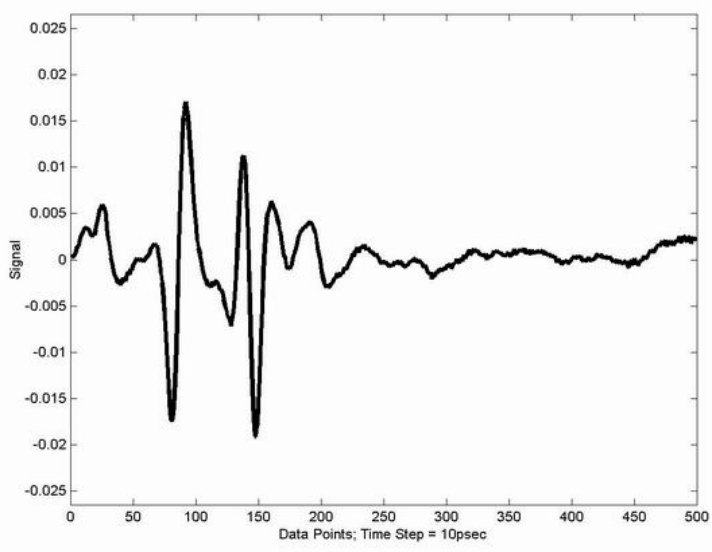
\includegraphics[height=0.4\textwidth]{2-LiteratureReview/A-scan.PNG}}
& \subfloat[B-scan]{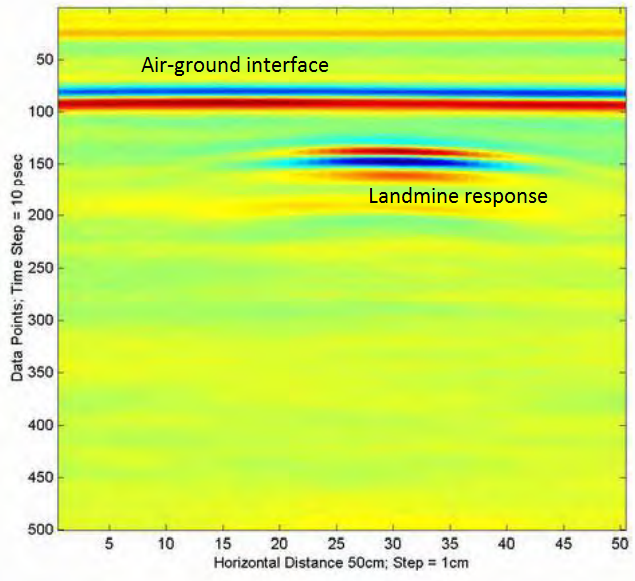
\includegraphics[height=0.4\textwidth]{2-LiteratureReview/B-scan.png}}\\
\end{tabular}}
\caption[Sample GPR response over buried anti-personnel mine]{Sample GPR response over a buried anti-personnel mine. An A-scan (a) is obtained from a stationary measurement, while a series of A-scans obtained by scanning in a line can be compiled (b) to form a B-scan \parencite{lee00}} 
\figlabel{GPRsample}
\end{figure}

The easiest way to detect an object is if the approximate response is previously known, such as from a model or training data set \parencite{Yarovoy2009}. Algorithms have been developed which identify pattern matches between a known expected response and the received response from the GPR. The most popular algorithm for this application is the inverse-matched filter, which is a mathematical convolution over the received signal to detect the presence of the expected response \parencite{Osumi1984}. More advanced algorithms are capable of producing results with greater accuracy when correlated with detection confidences from nearby samples. If a number of samples in a local area show high confidence in a detected object, the overall confidence that a detection has occurred increases when compared to an isolated positive detection. The hyperbola detection method identifies the hyperbolic shapes formed in a B-scan (as in \Figref{GPRsample}), through the use of computer vision techniques such as edge detection and the randomised Hough transform \parencite{Xu1990}.

% These algorithms represent the initial detection stage of the processing chain. Further classification of objects to reduce false-positive testing is possible through artificial intelligence strategies such as neural networks or decision trees, which require extensive sets of training data to produce strongly confident results, or through the pairing of the GPR detection with detection confirmation from a secondary sensor, such as a metal detector.

\section{Sensor fusion for landmine detection}
The wide range of potential materials, shapes and burial depths of landmines, as well as the constraints of sensing technologies, means that single sensor systems are limited in their detection capacity \parencite{Yarovoy2009}. Combination sensing through sensor fusion allows access to a wider range of information about a particular subsurface object, in turn allowing detection of a wider range of objects with heightened confidence. 
%Two potential configurations exist - where a single sensor is used as a primary detector with confirmation provided by secondary sensor, and where both sensors are used concurrently and information from both detectors is processed simultaneously. Mutual processing of the data from both sensors is called sensor fusion. 
A common distinction is made between potential levels of sensor fusion \parencite{Yarovoy2009}:
\begin{itemize}
\item \textbf{Decision-level fusion}: Information from the sensors is evaluated individually and a decision is made (landmine or non-landmine) for each sensor. Confidence in the sensor's independent decision is compared against a decision vector to produce a final determination.
\item \textbf{Feature-level fusion}: Information from the sensors is produced from the raw sensor data individually. This information is then combined from all sensors to create a singular feature, with a single and final determination made against this feature. 
\item \textbf{Data-level fusion}: Data is combined from all sensors to produce a single set of information about the feature. A final determination is made against this feature.
\end{itemize}
%Each progressive step down from decision-level fusion requires significantly greater computational processing, and greater knowledge of the sensor dynamics and the correlations of signal features to real-world object parameters \parencite{Yarovoy2009}. Higher level fusion strategies lend themselves well to machine learning techniques, which can be naive to the sensor mechanics and produce correlations based on learned sample data sets computationally cheaply. 
Experimental trials suggest that all forms of sensor fusion are capable of producing significantly more accurate detection results with far fewer false-positive incidents than single sensor systems \parencite{Yarovoy2009}. 

\textcolor{red}{Add more references, more details about achievements, sensor fusion results achieved by other people}
\section{Navigation}
\seclabel{navigationandautomation}
A major challenge associated with the automation of a platform is the development of software for control and navigation. Two aspects of this are how the platform tracks a path, and how it performs turning manoeuvres. 

\subsection{Path tracking}
\seclabel{pathTrackingLitReview}
Path tracking uses location information from a GPS or some other positioning system to guide a vehicle along a pre-defined course. In theory, the path can be defined as a continuous function, but this is inefficient in practice. Instead, a path is usually discretised and defined by a series of points, called waypoints (shown in \Figref{pathDefining}). Such a path can either be described as lines connecting the waypoints or as a series of closely spaced waypoints \parencite{Giesbrecht2005}.

\begin{figure}[htbp]
\centering
\subfloat[Continuous path]{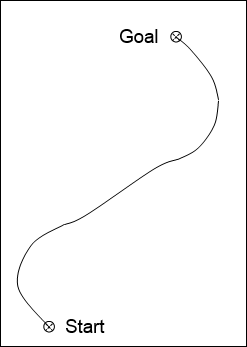
\includegraphics[width=0.28\textwidth]{2-LiteratureReview/pathContinuous.png}}\hspace{1em}%
\subfloat[Piecewise linear path]{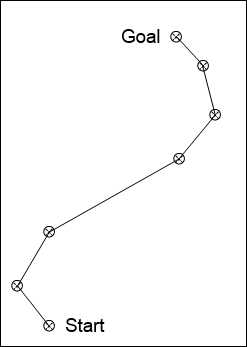
\includegraphics[width=0.28\textwidth]{2-LiteratureReview/pathPiecewise.png}}\hspace{1em}%
\subfloat[Set of discrete path nodes]{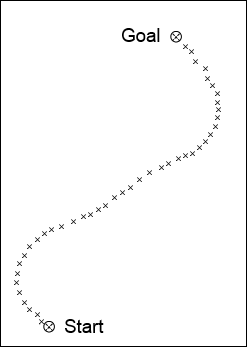
\includegraphics[width=0.28\textwidth]{2-LiteratureReview/pathDiscrete.png}}
\caption[Various ways to define a path]{Various ways to define a path \parencite{Giesbrecht2005}}
\figlabel{pathDefining}
\end{figure}

\subsubsection{Geometric path tracking}
Geometric path tracking uses geometric relationships between a vehicle and a path to produce a control algorithm as a solution to the problem. Theories assume vehicles use the Ackermann method for steering, so that a simplified steering model can be used for the geometry. This reveals a relationship between the steering angle and the curvature that the non-steering wheels will follow. Two of the most commonly used geometric vehicle models are Pure Pursuit and the Stanley method \parencite{snider2009}.

Pure Pursuit uses a path ``look-ahead'' distance to measure the future error between the vehicle and the path in real time, which can then be steered to and corrected for. \Figref{purePursuitGeom} shows the geometry associated with Pure Pursuit at one point in time. It shows a goal point $(g_x, g_y)$ on the desired path at a specified look-ahead distance $l_d$ in front of the vehicle. The steering angle is calculated based on an arc that would connect the centre of the non-steering axle to the goal point. The calculation of the goal point is effectively adding a waypoint to the path at that point. When high curvatures are present in a path, the controller may begin to cut corners due to a look-ahead distance that would effectively skip this portion of the path. Lateral error on a path of constant curvature may also be experienced due to geometric controller characteristics which do not take into account the curvature of a path. However, Pure Pursuit provides a very robust tracking algorithm when discontinuous curvatures are present \parencite{snider2009}. In general, for more accurate tracking a short look-ahead distance should be used but will eventually result in oscillation, for smoother tracking a long look-ahead distance should be used but this will reduce precision \parencite{snider2009}.
\begin{figure}[ht]
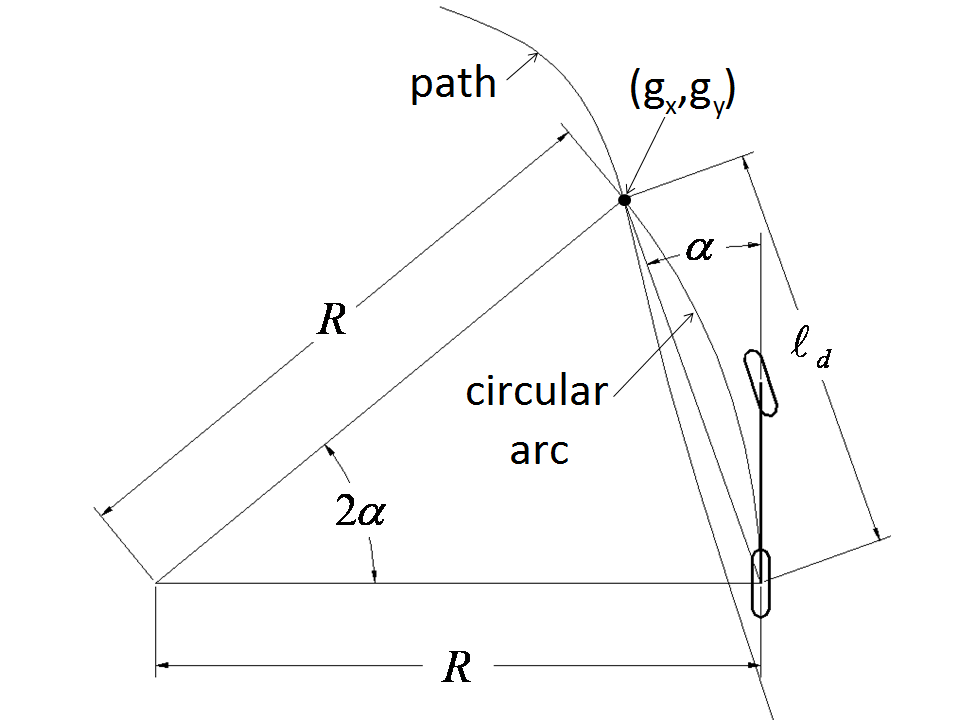
\includegraphics[width=0.6\textwidth]{2-LiteratureReview/purePursuitGoal.png}
\centering
\caption[Pure Pursuit geometry]{Pure Pursuit geometry \parencite{snider2009}} \figlabel{purePursuitGeom}
\end{figure}

%\nomenclature[S]{$l_d$}{Pure Pursuit model look ahead distance}%
%\nomenclature[S]{$(g_x, g_y)$}{Pure Pursuit model goal point}%

Unlike Pure Pursuit which is based on the future error, the Stanley method uses the current lateral error between the centre of a wheel's axle and the nearest path point (\Figref{stanleyGeom}). The desired effect is that as the vehicle strays further from the path, the wheel's steering angle is amplified in an attempt to correct for the error. The Stanley method is very well suited to higher speed tracking but can run into problems when curvature discontinuities are present in the path. The model sets the steer angle to the heading error, which is calculated as the difference between the vehicle's heading and the instantaneous heading of the nearest point on the path, $\theta_e$. An extra term is used when the lateral error is non-zero which amplifies the steer angle to a new value of $\delta$.
\begin{figure}[ht]
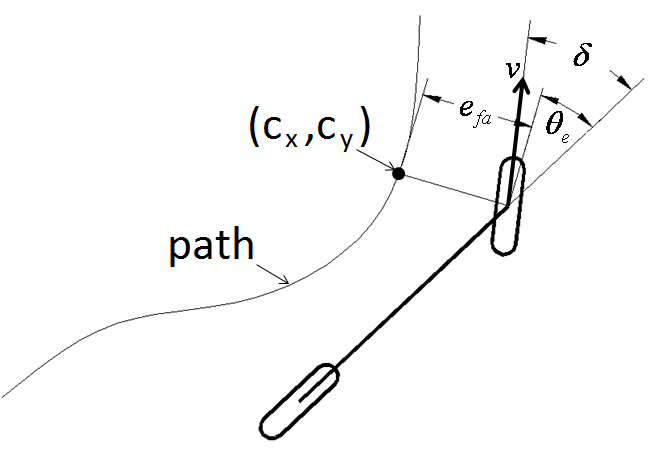
\includegraphics[width=0.5\textwidth]{2-LiteratureReview/stanleyMethod.png}
\centering
\caption[Stanley method geometry]{Stanley method geometry \parencite{snider2009}} \figlabel{stanleyGeom}
\end{figure}

%\nomenclature[S]{$\theta_e$}{Stanley method heading error}%
%\nomenclature[S]{$\delta$}{Steering angle}%

Some limitations of geometric path tracking methods are related to the dynamics of a vehicle which are not present in the theory, namely the capabilities of a platform and its actuators. Due to this, the method expects an instant response from elements such as the steering, which is an issue when high path curvatures are present or when the curvature of the path suddenly changes. As a result, the method cannot guarantee that the vehicle will follow a path as accurately as designed and at high speeds that vehicle may skid or tip \parencite{coulter1992}.

\subsubsection{Kinematic path tracking}
The kinematic model collapses a four wheeled vehicle into a two wheeled model, much like the geometric path tracking approach. The equations of motion for the simplified system are then used to relate the vehicle speed, change in heading error and change in lateral error to a user defined velocity and steer angle in path coordinates. In practice, the same trade off between performance and stability is apparent as in the geometric models, tracking accuracy declines at high speeds due to neglected dynamics \parencite{snider2009}. This method is not as robust as Pure Pursuit and displays a similar behaviour to the Stanley method when discontinuities in curvature are present.
\subsubsection{Dynamic path tracking}
A dynamic model approximates the real dynamics of a vehicle, which was one of the downfalls of the previous examples. Similar to the kinematic model, the vehicle speed, heading error and lateral error are related to a user defined velocity and steer angle in path coordinates. Even though the dynamics of the vehicle are included in this model, extreme path properties such as large changes in curvature can have a very large effect on the accuracy and efficiency of the path tracking \parencite{snider2009}. Discontinuities in the path still have a noticeable effect on accuracy, and the steady state lateral error is still present. However, in a more realistic scenario a dynamic path tracking method does show overall improvement \parencite{snider2009}.

\subsection{Performing turning manoeuvres}
%maybe move this section to concept or detailed design AFTER we have established that our area subdivision is primarily linear. can then talk about it in more detail
In a path similar to that described by the piecewise linear definition, a turn can be moderately controlled by introducing a variable called the radial tolerance \parencite{Giesbrecht2005}. The radial tolerance describes the distance from the waypoint at which the system considers that waypoint 'reached', ultimately changing the point at which the platform will begin the turn towards the proceeding waypoint. If the radial tolerance is set too large the platform will begin the turn early resulting in poor path tracking. If the radial tolerance is set too small the platform will overshoot the desired path due to unaccounted vehicle dynamics and/or restrictions in steering angle. \Figref{waypointTolerances} shows examples of a radial tolerance set slightly too low at 1 metre, denoted by the plus signs, and more realistically at 6 metres, denoted by the circles, for a vehicle following the path a rectangular path with a turn radius of 4 metres. It is clearly visible that both methods are unable to follow the desired path, shown as a solid line, with perfect precision due to real vehicle dynamics.
\begin{figure}[ht]
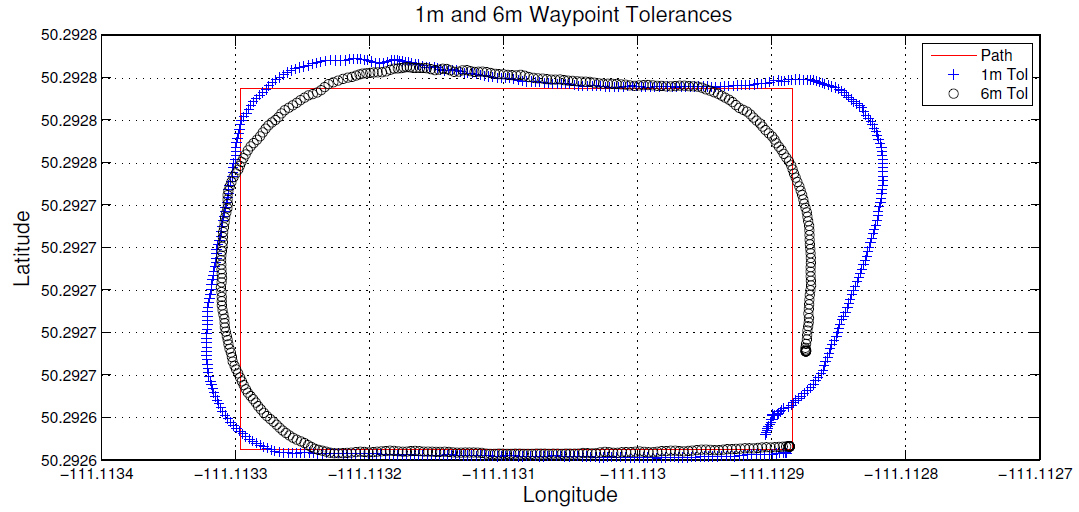
\includegraphics[width=\textwidth]{2-LiteratureReview/waypointTolerances.PNG}
\centering
\caption[Effect of waypoint tolerances on path tracking]{Effect of waypoint tolerances on path tracking \parencite{Giesbrecht2005}} \figlabel{waypointTolerances}
\end{figure}

\textcolor{red}{This section (automation and navigation) needs more examples of what others have been able to achieve, rather than just listing advantages of various methods}
\section{Outcomes}
\textcolor{red}{Maz said we need a section at the end of the lit review on the decisions (i.e. we did the whole lit review, now what are the things we decided to use or apply to our project (I think?))}
The literature review covered different methods for signal processing, sensor fusion and platform navigation. The phase plot signature method was found to be an effective way to characterise landmines in metal detector data, based on the metrics of phase angle and magnitude. GPR signal processing on the other hand is much more complicated, with the received signals being strongly affected by the soil conditions, thus highlighting the need for a preprocessing routine. Target characterisation can be achieved be analysing features of the A-scan or B-scan. Several methods were also explored for path tracking and turning,... 

\end{document}